\section*{Loss system: Erlang-B distribution} \label{ex_1}

\subsection*{Resultados da Simulação}

\begin{figure}[H]
    \centering
    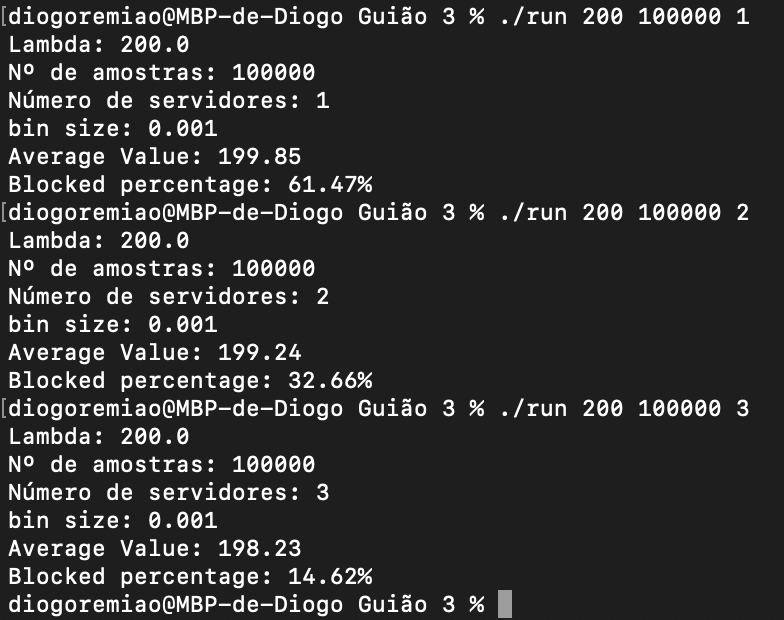
\includegraphics[width=.8\linewidth]{figs/image_1.png}
    \caption{Simulação para diferentes números de servidores}
    \label{fig:1}
\end{figure}

A simulação foi feita com os parâmetros \textit{Arrival Rate}=200 e \textit{Service Rate}=0.008 indicados no guião.

O número de amostras simuladas foi 100.000, que se provou um bom equilíbrio entre fidelidade dos resultados e tempo de simulação.

O parâmetro \textit{Number of servers} é inserido durante a execução do script para ser mais fácil simular diferentes valores.

\subsection*{Resultados teóricos}

\begin{figure}[H]
    \centering
    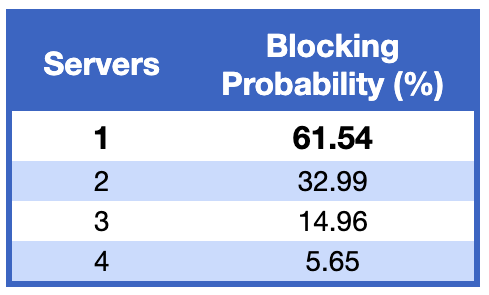
\includegraphics[width=.5\linewidth]{figs/image_2.png}
    \caption{Valores esperados no site}
    \label{fig:2}
\end{figure}

Ao comparar os valores obtidos com os esperados, observamos que a diferença é mínima, quer para a percentagem de bloqueio, quer para a estimação do Lambda.
Como esperado, se estiverem disponíveis mais servidores para processar os pacotes, a percentagem de bloqueio é menor.

\section*{Waiting system with infinite length queue: Erlang-C distribution} \label{ex_2}

\subsection*{Resultados da Simulação}

\begin{figure}[H]
    \centering
    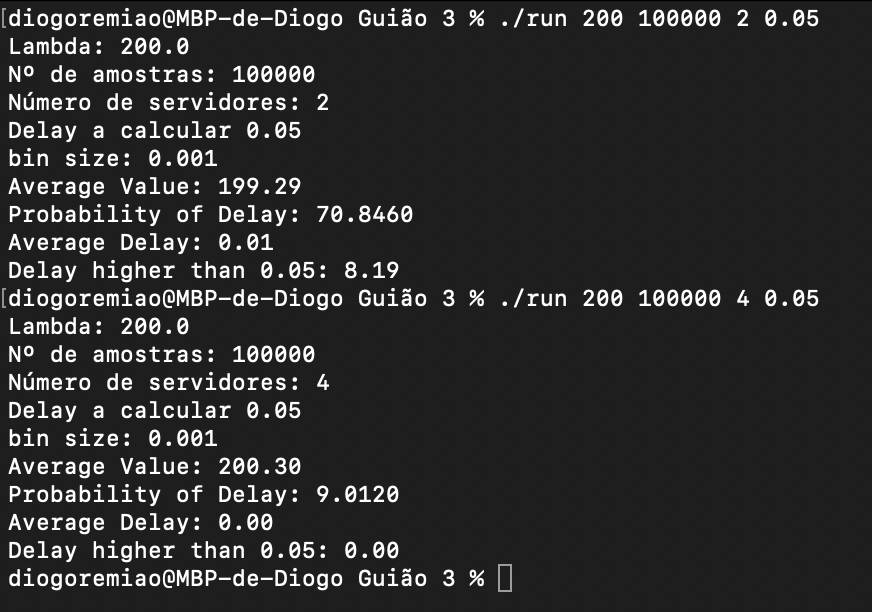
\includegraphics[width=.5\linewidth]{figs/image_3.png}
    \caption{Simulação para diferentes números de servidores}
    \label{fig:3}
\end{figure}

A simulação foi feita com os parâmetros mesmos parâmetros.
Foi escolhido o valor 0.05 para calcular a percentagem de atrasos acima de valor, onde se obteu como esperado uma percentagem mais alta quando o número de servidores é menor.

\subsection*{Resultados teóricos}

\begin{figure}[H]
    \centering
    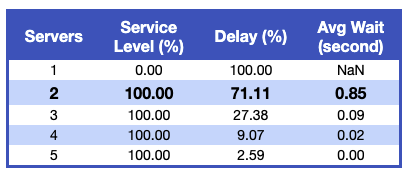
\includegraphics[width=.5\linewidth]{figs/image_4.png}
    \caption{Valores esperados no site}
    \label{fig:4}
\end{figure}

Para apenas um servidores disponível, não é possível processar os pacotes que estão a chegar em tempo real.
Isto leva a uma fila de espera "infinita" e consequentemente, uma percentagem de atraso de 100\%.

Estando disponíveis mais servidores, menos vão ser colocados na fila de espera.
Quando mais servidores, menos tempo estes têm que esperar para serem atendidos.

\begin{figure}[H]
    \centering
    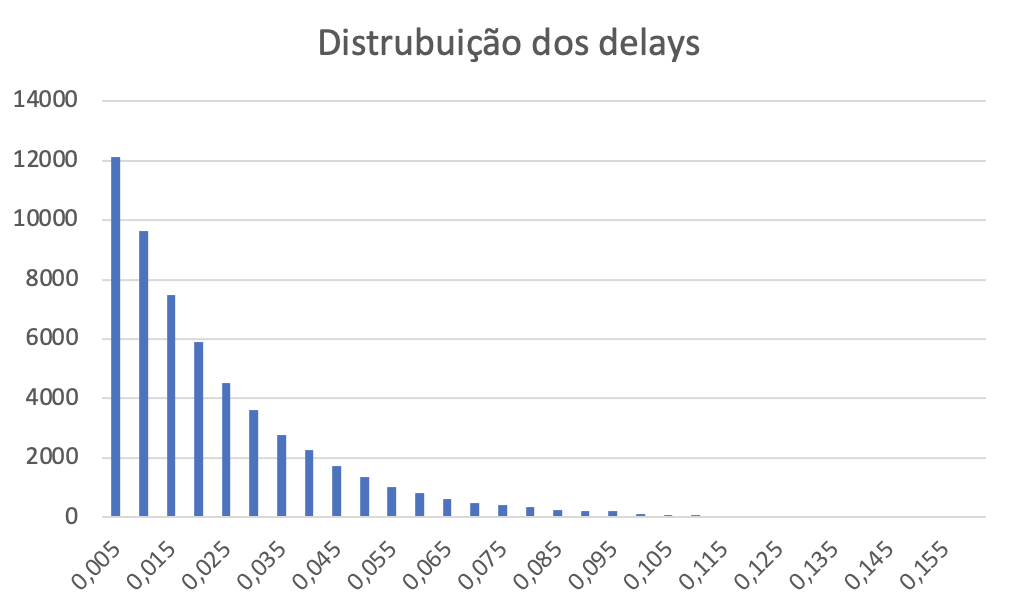
\includegraphics[width=.8\linewidth]{figs/image_8.png}
    \caption{Histograma dos delays}
    \label{fig:8}
\end{figure}

O histograma apresenta uma distribuição exponencial para os delays > 0, estando de acordo com a distribuição exponencial dos tempos de chegada.

\section*{General case –waiting system with finite length queue} \label{ex_3}

\subsection*{Resultados da Simulação - Erlang B / Erlang C com fila de espera infinita}

\begin{figure}[H]
    \centering
    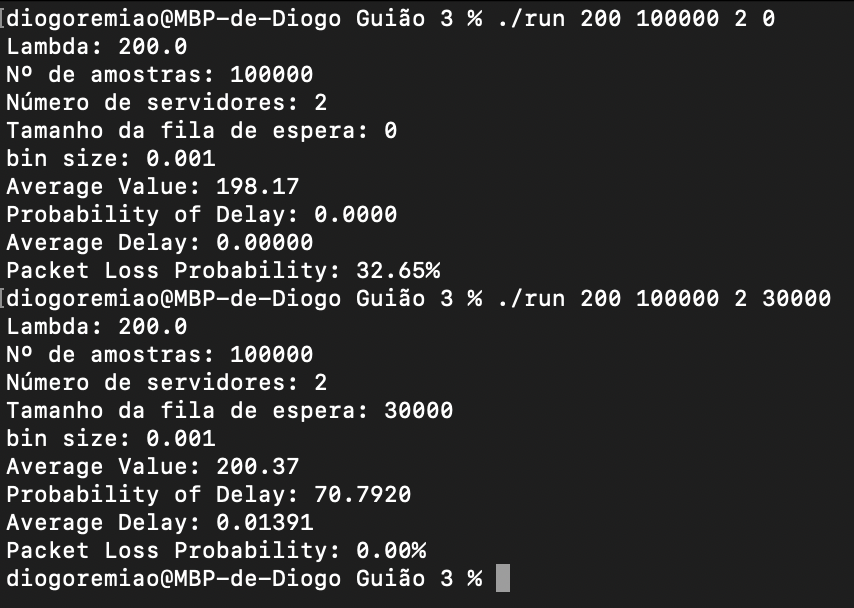
\includegraphics[width=.8\linewidth]{figs/image_5.png}
    \caption{Resultados com fila de espera de tamanho 0 / arbitrariamente grande}
    \label{fig:5}
\end{figure}

Para simular o caso de Erlang B, definimos o tamanho da fila como 0. Deste modo, o pacote que chega ou é servido ou é eliminado.
É o mesmo cenário da secção \ref{ex_1}. Como podemos observar, obtemos os mesmos resultados como indicado na figura \ref{fig:2}.
Deste modo podemos confirmar o correto funcionamento do simulador geral no caso de Erlang B.

Por outro lado, também é possível simular o caso de Erlang C com fila infinita.
Apesar de não ser possível definir um valor infinito para a fila, podemos escolher um valor proporcionalmente grande ao número de amostras simuladas.
Neste caso definimos a fila com tamanho de 30.000. Mais uma vez faz-se o paralelismo com a simulação da secção \ref{ex_2}.
Ao analisarmos os resultados obtidos e compararmos com a figura \ref{fig:4}, observamos que mais um vez estão de acordo com os valores esperados.

\subsection*{Resultados da Simulação - Erlang C com fila de espera de tamanho L}

\begin{figure}[H]
    \centering
    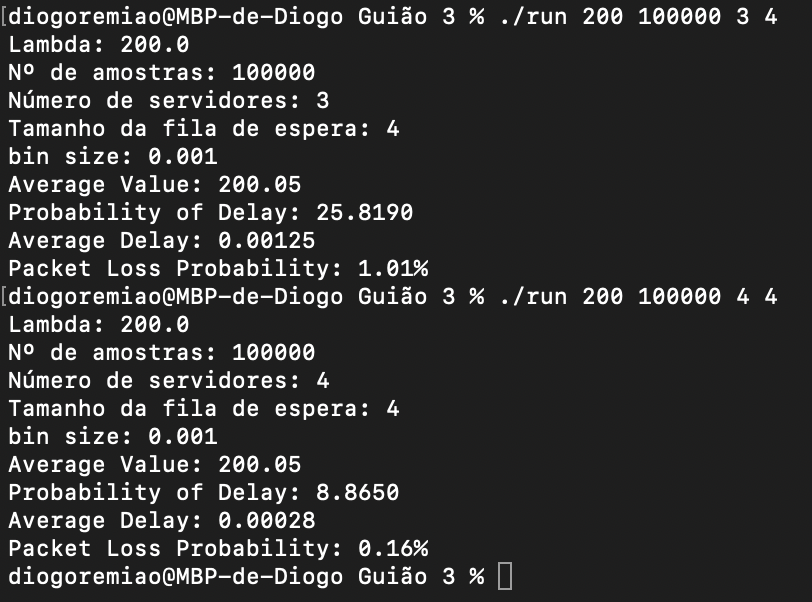
\includegraphics[width=.8\linewidth]{figs/image_6.png}
    \caption{Resultados com fila de espera de tamanho 4}
    \label{fig:6}
\end{figure}

Este simulador também permite simular com filas de tamanho finito.
Como indicado pelo guião, foi calculado por método iterativo os valores de N (servidores) e L (fila de espera) que produzem um percentagem de pacote perdido de 1\%.
Fizemos esta simulação para diferentes combinações de servidores e tamanhos de filas.
Obtemos os seguintes resultados (N,L): (2,13), (3,4) e (4,2).
NA figura \ref{fig:6} está representado o para a simulação (3,4).
Foi também simulado para (4,4) para demonstrar que com mais servidores, a percentagem de perda e de atraso diminui.


\subsection*{Resultados teóricos}

\begin{figure}[H]
    \centering
    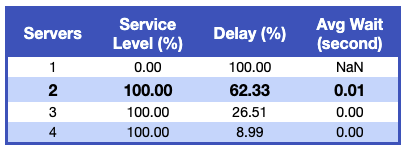
\includegraphics[width=.5\linewidth]{figs/image_7.png}
    \caption{Valores esperados no site}
    \label{fig:7}
\end{figure}

Quando comparando com valores indicados no website, notamos um discrepância maior de resultados, especialmente para N/L mais pequenos.
Isto deve-se ao facto de o valor de \textit{Delay} no website incluir também o valor de pacotes perdidos.
Deste modo, para perdas muito baixas, a diferença é muito pequena e vise-versa.

Como podemos observar, para (3,4), o \textit{Delay} é de 25.8\% e \textit{Packet Loss} de 1\%.
A soma dá aproximadamente o valor obtido no website de 26.5\%.

Quando o valor de \textit{Packet Loss} é menor (4,4), a diferença é mais pequena $8.86\% + 0.16\%$, com um resultado proximo de 8.99\%.
